\documentclass[14pt,a4paper]{extarticle}
\usepackage[utf8]{inputenc}
\usepackage[russian]{babel}
\usepackage{amsmath}
\usepackage{amsfonts}
\usepackage{amssymb}
\usepackage{setspace}
\usepackage[left=2.5cm, right=2cm, bottom=1.5cm, top=2cm]{geometry}
\usepackage{indentfirst}
\usepackage{tikz}
\usepackage{siunitx}
\usepackage{caption}
\usepackage{listings}
\usepackage{graphicx}

\newcommand{\pd}[2]{\frac{\partial #1}{\partial #2}}
\newcommand{\dpd}[2]{\dfrac{\partial #1}{\partial #2}}

\newcommand{\pdd}[2]{\frac{\partial^2 #1}{\partial #2^2}}
\newcommand{\pddd}[3]{\frac{\partial^2 #1}{\partial #2\partial #3}}

\renewcommand{\arraystretch}{1.2}

\let\dividesymbol\div
\renewcommand{\div}{\operatorname{div}}
\newcommand{\grad}{\operatorname{grad}}
\newcommand{\rot}{\operatorname{rot}}
\newcommand{\const}{\operatorname{const}}
\newcommand{\diag}{\operatorname{diag}}
\renewcommand{\vec}[1]{\boldsymbol{\mathbf{#1}}}
\newcommand{\ten}[1]{\mathbf{#1}}
\newcommand{\cutefrac}[2]{{}^{#1}\mkern-5mu/{\!}_#2}
\newcommand{\half}{{\cutefrac{1}{2}}}
\renewcommand{\leq}{\leqslant}
\renewcommand{\geq}{\geqslant}

\newcommand{\n}[1]{\num[exponent-product=\cdot]{#1}}

\begin{document}
\begin{center}
	Московский физико-технический институт (Государственный университет)\\
Факультет управления и прикладной математики\\
	\vspace{1cm} Моделирование многофазных реагирующих фильтрационных течений с 	равновесными химическими реакциями.\\
	\vspace{1cm}Выпускная квалификационная работа на степень бакалавра\\
			\vspace{1cm}студента 373 группы\\
	\vspace{1cm}Гринина Виктора Олеговича
	\vspace{4cm}
\end{center} 

\onehalfspacing

\clearpage
\tableofcontents
\clearpage

\section{Введение}

В настоящей работе рассматриваются многофазные фильтрационные течения, в которых наряду с реакциями с конечной кинетикой присутствуют равновесные химические реакции. Для описания данного процесса используются система уравнений, описывающая  многофазное фильтрационное течение, и система уравнений, описывающая процесс установления химического равновесия. Системы решаются последовательно на каждом шаге по времени. Сначала, с помощью симулятора многофазных фильтрационных течений, решается первая из них. Полученные результаты используются в качестве начальных приближений для второй системы.   
$$\tikz{
\fill[fill=yellow]
   (0,0) node[fill=yellow!20,draw,double,rounded corners] {Равновесные химические реакции}
   -- (0,4) node[fill=yellow!20,draw,double,rounded corners] {Многофазное фильтрационное течение};
   \draw [->, red] (1, 1) -- (1,3);
   \draw [->, blue] (-1,3) -- (-1,1);
}$$

Цель работы заключалась в написании модуля для решения задачи о фазовом равновесии и добавлении его к имеющемуся программному комплексу, для проведения численных экспериментов.

\section{Математическая модель}

\subsection{Уравнения химических реакций}

Основными уравнениями, которые описывают течение многофазной многокомпонентной среды являются уравнения балансов количества вещества и энергии, имеющие вид
\begin{gather*}
\pd{N_i}{t} + \div \vec Q_i = \vec S_i,\\
\pd{E}{t} + \div \vec J = \vec R.
\end{gather*}
Здесь $N_i$ --- молярные концентрации компонент, $E$ --- плотность энергии среды. Химические реакции учитываются в математической модели течения многофазной многокомпонентной среды в виде источников количества вещества $S_i$ и энергии $R$.

Для реакций с конечной скоростью обычно используется закон Арениуса, когда скорость реакции пропорциональна концентрациям реагирующих веществ в степенях их стехеометрических коэффициентов.
В случае равновесной химической реакции вместо скорости реакции имеется равновесное соотношение
$$F(N_i) = 0,$$
выражающее собой равенство скоростей прямой и обратной химических реакций.

Если записать равновесную химическую реакцию в виде 
$$\sum{\nu_i X_i} \rightleftharpoons 0,$$
где $X_i$ --- реагирующие вещества, а $\nu_i$ --- их стехеометрические коэффициенты в реакции, то для такой реакции принимается верным закон действующих масс:
$$
K = \prod_i N_i^{\nu_i}.
$$
Здесь предполагается, что $\nu_i$ для продуктов реакции положительны, а для реагентов --- отрицательны. В качестве функции $F$ для данной реакции можно взять 
$$F = \ln{K} + \sum{\nu_i \ln{N_i}}.$$
Пусть в силу  некоторых причин, например из-за переноса продуктов реакции течением, данное равновесие оказалось нарушено. Пусть начальные концентрации $N_i^0$. Тогда из-за данной реакции концентрации изменяются по закону $$\Delta N_i = \xi \nu_i,$$ где $\xi$ --- величина, характеризующая глубину реакции, одинаковая для всех участвующих компонент.

Задача определения нового равновесия заключается в поиске такого значения $\xi$, что $F(N_i) = 0$. При этом, можно сделать очевидное обобщение на случай нескольких реакций
\begin{gather*}
N_i = N_i^0 + \sum_{j=1}^{M} \xi_j\nu_{i,j}\\
F_j(N_i)=\ln(K_j) + \sum_{i=1}^{M} \nu_{i,j}\ln{N_i} = 0
\end{gather*}
 
\subsection{Конкретные химические реакции}

\newcommand{\OHm}{\text{OH}^-}
\newcommand{\Hp}{\text{H}^+}
\newcommand{\WAT}{\text{H}_2\text{O}}
\newcommand{\CARB}{\text{CO}_2}
\newcommand{\Catwop}{\text{Ca}^{2+}}
\newcommand{\Calcite}{\text{CaCO}_3}
\newcommand{\HCO}{\text{HCO}_3^{-}}
При проведении расчётов использовалась следующая система химических реакций
\begin{align*}
R1:&\quad \OHm + \Hp \rightleftharpoons \WAT,\\
R2:&\quad \HCO +\Hp \rightleftharpoons \WAT + \CARB,\\
R3:&\quad \Calcite + 2\Hp \rightleftharpoons \WAT + \CARB + \Catwop.
\end{align*}

Эта  система может быть записана в матрично-векторной форме $V^T Y \rightleftharpoons 0$, где
$$V^T =  \begin{Vmatrix}
-1 &0 &0  &1 &0 &-1 &0\\
0 &-1 &0  &1 &1 &-1 &0\\
0  &0 &-1  &1 &1 &-2 &1
		\end{Vmatrix}, \quad
  Y = \begin{Vmatrix}
  \OHm\\
  \HCO\\
  \Calcite\\
  \WAT\\
  \CARB\\
  \Hp\\
  \Catwop
  \end{Vmatrix}$$\\
Или в виде таблицы Мореля\\
$$\begin{array}{|c|cccc|c|}
\hline
		&\WAT	&\Hp	&\CARB	&\Catwop	&\lg {K}\\
\hline
\OHm		&1		&-1		&0		  &0		&-14\\
%\hline
\HCO	&1		&-1		&1		  &0		&-5.928\\
%\hline
\Calcite		&1		&-2		&1		  &1		&-8.094\\
\hline
\end{array}$$

\section{Численный метод и программный модуль}

Для решения системы, которая описывает установление химического равновесия, использовался метод Ньютона. Были рассмотренные различные способы записи данной системы и был выбран оптимальный.

Запишем приведённую раньше систему в матричной форме$$\vec{F}(\vec \xi) = \ln{\vec{K}} + V^T \ln{(\vec{N}^0 + V\vec \xi)} = 0$$
Продифференцируем эту функцию по $\vec \xi$
$$\frac{\partial \vec{F}}{\partial{\vec{\xi}}} = V^T\diag^{-1}(\vec{N}^0 + V\vec{\xi})V$$

Метод Ньютона принимает вид
$$\vec{\xi}^{k+1} = \vec{\xi}^{k} - \alpha^{(k)}[V^T\diag^{-1}(\vec{N}^0 + V\vec{\xi})V]^{-1}(\ln{\vec{K}} + V^T \ln{(\vec{N}^0 + V\vec{\xi})}) \quad (1)$$
Для обычного метода Ньютона параметр $\alpha$ следует брать равным единице, однако итерации с $\alpha^{(k)} = 1$ могут привести к попаданию в область нефизических значений. В этом случае можно делать лишь часть шага метода Ньютона, выбирая параметр $\alpha$ из промежутка $[0, 1]$.   

При применении данного метода для численных расчётов возникает несколько проблем. Нужно выбирать начальное приближение $\vec{\xi}^0$ так, чтобы выражение под логарифмом было положительным $\vec{N}^0 + V\vec{\xi} > 0$. Для чего нужно решать систему неравенств. Кроме того на каждой итерации следует задавать параметр $\alpha^{(k)} \in [0,1]$ так, чтобы неравенства этой системы не нарушались.  

\begin{verbatim}
 def choose_a(N0, V, reactionDepth, C):
    safe = 0.5
    a = 1 / safe
    N = N0 + V.dot(reactionDepth)
    dN = V.dot(C)
    for i in range(len(N)):
    	if (N[i] + a * dN[i] < 0):
    	a = -N[i]/dN[i]
    return a * safe
\end{verbatim}

Перепишем систему в другом виде, для этого введём дополнительные переменные $$\vec{p} = \ln{(\vec{N}^0 + V\vec{\xi})}$$ 

При этом получаем расширенную систему
$$\begin{cases} 
	\vec{F} = \ln{\vec{K}} + V^T\vec{p}=0,\\
	\exp(\vec{p})=\vec{N}^0 + V\vec{\xi};
	
\end{cases}$$
$$\begin{cases} 
	\ln{\vec{K}} + V^T\vec{p}=0,\\
	\vec{N}^0 + V\vec{\xi} - \exp(\vec{p}) = 0;
\end{cases}$$
Эта система полностью эквивалентна исходной. Её можно записать в виде
$\vec{\Phi}(\vec{x}) = 0$, где $ \vec{x} = [\vec{\xi}, \vec{p}]$

Тогда метод Ньютона принимает вид\\
$$\vec{x}^{k+1} = \vec{x}^{k} - \alpha^{(k)}\left(\pd{\vec{\Phi}}{\vec{x}}\right)^{-1}\vec{\Phi}(\vec x^k) \quad (2)$$
 где $$\pd{\vec{\Phi}}{\vec{x}} = \begin{Vmatrix}
 0 & V^T \\
 V & -\diag({\exp(\vec{p})})
\end{Vmatrix}  $$
Использование метода Ньютона переписанного в такой форме, уже не встречает проблем, характерных предыдущей версии. Как показывает эксперимент он сходится из любого начального приближения, при любых начальных концентрациях. Кроме того в данном случае можно выбрать $\alpha^{(k)} = 1$, что обеспечивает большую скорость сходимости.

Модуль, реализующий метод Ньютона в такой форме, был включён в симулятор многофазных фильтрационных течений. 


\section{Результаты}
\subsection{Верификация написанного модуля}
Приведём результаты расчётов системы из трёх химических реакций 
\begin{align*}
R1:&\quad \OHm + \Hp \rightleftharpoons \WAT,\\
R2:&\quad \HCO +\Hp \rightleftharpoons \WAT + \CARB,\\
R3:&\quad \Calcite + 2\Hp \rightleftharpoons \WAT + \CARB + \Catwop.
\end{align*}

Будем считать, что начальные концентрации всех ионов равнялась нулю и вектор концентраций химических веществ имел вид
$$\vec{N}_0^T = [0, 0, 1, 1, 1, 0, 0]$$

Для метода Ньютона записанного в форме $(1)$ начальное приближение искомых глубин реакции выбираем так, чтобы выполнялось условие $$\vec{N}^0 + V\vec{\xi} > 0.$$ Пусть например $$\vec{\xi}_0^T = [-0.5, -0.7, 0.5]$$ 
\begin{table}[ht!]
	\caption{Концентрации веществ и выбираемый параметр $\alpha$ на соответствующей итерации метода Ньютона записанного в форме $(1)$.}
	\small
	\begin{center}
	\begin{tabular}{|p{0.33cm}|p{1.7cm}|p{1.7cm}|p{1.7cm}|p{1.7cm}|p{1.7cm}|p{1.7cm}|p{1.7cm}|l|}
	\hline
		&$\OHm$	&$\HCO$ &$\Calcite$ &$\WAT$ &$\CARB$ &$\Hp$ &$\Catwop$ &$\alpha$\\
\hline
	1	&0	&0	&1  &1	&1	&0	&0	&0.05\\
%\hline
	2	&0.5	&0.7	&0.5 &0.3	&0.8 &0.06	&0.2	&0.06	\\
%\hline
	4	&0.12   &0.75  &0.60  &0.51 &0.63  &0.09 &0.39	&0.06\\
%\hline
	8	&\n{7.8e-03}   &\n{6.4e-01}  &\n{6.9e-01}  &\n{6.6e-01}  &\n{6.6e-01}  &\n{3.4e-02} &\n{3.1e-01}	&0.09\\
%\hline
	16	&\n{1.5e-05}   &\n{3.6e-01}   &\n{8.2e-01}   &\n{8.2e-01} &\n{8.2e-01}   &\n{3.3e-03}   &\n{1.8e-01}	&0.88\\
%\hline
	30	&\n{ 5.9e-10}    &\n{6.7e-02 }    &\n{9.7e-01 }    &\n{9.7e-01   } &\n{9.7e-01} &\n{1.6e-05  }  &\n{3.4e-02}	&1\\
\hline
	
\end{tabular}
\end{center}
\end{table}

Видим что в результате химических реакций концентрации исходных веществ немного уменьшаются, в результате чего образуются все входящие в реакции ионы. 

На начальных итерациях выбирается $\alpha < 1$. Это говорит о том, что метод Ньютона пытается выйти за допустимую область. В результате ограничения шага, в этом случае сходимость является линейной и метод Ньютона работает как метод простой итерации. 

Для расширенной системы, как уже говорилось, $\alpha$ выбирается равным единице. Начальные значения $\xi_i$ можно выбрать произвольными. Пусть они будут таким же как в предыдущем случае.
\begin{table}[ht!]
	\caption{Концентрации веществ на соответствующей итерации метода Ньютона записанного в форме $(2)$.}
	\small
	\begin{center}
	\begin{tabular}{|p{0.33cm}|p{1.7cm}|p{1.7cm}|p{1.7cm}|p{1.7cm}|p{1.7cm}|p{1.7cm}|p{1.7cm}|l|}
	\hline
		&$\OHm$	&$\HCO$ &$\Calcite$ &$\WAT$ &$\CARB$ &$\Hp$ &$\Catwop$ \\
\hline
	1	&0	&0	&1  &1	&1	&0	&0	\\
%\hline
	2	&\n{0.7}	&\n{1.9}	&\n{0.3}	&\n{0.8}	&\n{0.5}	&\n{1.0}	&\n{1.0}	\\
%\hline
	4	&\n{6.0e-09}      &\n{1.7}      &\n{3.6}      &\n{4234.8}    &\n{2.3} &\n{7e-03}      &\n{2.2}\\
%\hline
	8	&\n{2.6e-09}    &\n{2.6e-01}   &\n{8.7e-01}      &\n{78.1}    &\n{8.7e-01} &\n{3.1e-04 }     &\n{1.5e-01}\\
%\hline
	12	 &\n{7.6e-10}    &\n{8.6e-02 }    &\n{9.6e-01 }     &\n{ 2.1  }   &\n{9.6e-01} &\n{2.7e-05}    &\n{4.3e-02}\\
%\hline
	16	&\n{ 5.9e-10}    &\n{6.7e-02 }    &\n{9.7e-01 }    &\n{9.7e-01   } &\n{9.7e-01} &\n{1.6e-05  }  &\n{3.4e-02}\\
\hline
	
\end{tabular}
\end{center}
\end{table}

Оба варианта метода Ньютона сходятся к одному и тому же значению. При этом второй из них требуется меньшее количество итераций.
\subsection{Применение модуля в симуляторе}
Разработанный алгоритм был включён в симулятор и использован для моделирования многофазных фильтрационных течений с химическими реакциями.

Одним из верификационных сценариев расчёта стала следующая задача. В данной задаче рассматривается вытеснение углекислым газом($\CARB$) воды($\WAT$) из пористой области, скелет которой составляет углекислый кальций($\Calcite$). 

Геометрия задачи такова
$$
\tikz {


\draw (0,0) --  +(10,0) -- +(10,2) -- +(0, 2) -- +(0,0);
\filldraw[fill=blue!20!white, draw=blue] (1,0) --  (16,0) -- (16,2) -- (1, 2) -- (1,0);
\filldraw[fill=blue!5!white, draw=blue] (0,0) --  (1,0) -- (1,2) -- (0, 2) -- (0,0);
\draw[dashed, gray] (0,0.25) -- (16,0.25); 
\draw[dashed, gray] (0,0.5) -- (16,0.5); 
\draw[dashed, gray] (1,0.75) -- (15,0.75); 
\draw[dashed, gray] (1, 1) -- (15, 1);
\draw[dashed, gray] (1,1.25) -- (15,1.25); 
\draw[dashed, gray] (0,1.5) -- (16,1.5); 
\draw[dashed, gray] (0,1.75) -- (16,1.75);

\draw[dashed, gray] (1,0) -- (1,2); 
\draw[dashed, gray] (2,0) -- (2,2); 
\draw[dashed, gray] (3,0) -- (3,2); 
\draw[dashed, gray] (4,0) -- (4,2); 
\draw[dashed, gray] (5,0) -- (5,2); 
\draw[dashed, gray] (6,0) -- (6,2); 
\draw[dashed, gray] (7,0) -- (7,2); 
\draw[dashed, gray] (8,0) -- (8,2);
\draw[dashed, gray] (9,0) -- (9,2);
\draw[dashed, gray] (10,0) -- (10,2); 
\draw[dashed, gray] (11,0) -- (11,2); 
\draw[dashed, gray] (12,0) -- (12,2); 
\draw[dashed, gray] (13,0) -- (13,2); 
\draw[dashed, gray] (14,0) -- (14,2); 
\draw[dashed, gray] (15,0) -- (15,2);

\draw [<->, orange] (0, -0.9) -- (16, -0.9); 
\draw [->, blue!20!white] (0, 2.2) -- (1, 2.2);
\fill
(0.5,1) node {inj}
(15.5,1) node {prod} 
(8,-0.6) node {L}
(0.5, 2.5) node {$\CARB$}
}
$$
Имеется одномерная область длины $L$. Пунктирной линией схематично показаны поры скелета, занятые водой. На концах области находятся скажины: cлева - нагнетающая$(inj)$, справа - добывающая скважина $(prod)$. Начальная температура в области $20^\circ C$, начальное давление $100$ атмосфер.

Нагнетающая скважина закачивает в область углекислый газ при постоянном давление $101$ атмосфера, который постепенно вытесняет из области воду и частично растворяется в ней. Перенос жидкости и газа сопровождается химическими реакциями описанными в предыдущих пунктах, в результате чего скелет распадается и вымывается из области.

\begin{figure}[h!]
\includegraphics[width=1\textwidth]{pic1}
\caption{Концентрация скелета в различных участках области} \label{fig:pic1}
\end{figure}

Так как пористость среды определяется просто как $\frac{V_{\text{пор}}}{V} = \frac{1 - V_{\text{скел}}}{V}$, то в результате распада скелета она увеличивается. В освобождающееся пространство устремляется поток углекислого газа и воды. 

\begin{figure}[h!]
\includegraphics[width=1\textwidth]{pic2}
\caption{Концентрация воды в различных участках области. Зелёным для потока с химическими реакциями, синим для потока без химических реакций} \label{fig:pic1}
\end{figure}

\begin{figure}[h!]
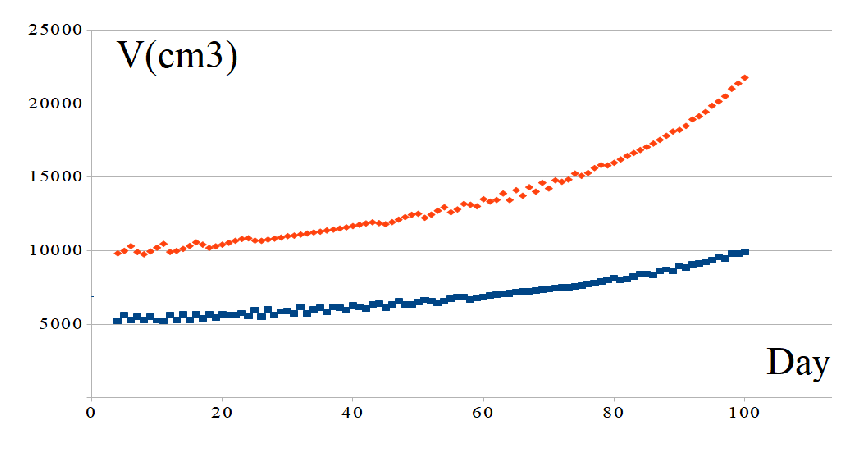
\includegraphics[width=1\textwidth]{pic3}
\caption{Расход углекислого газа через нагнетающую скважину} \label{fig:pic1}
\end{figure}


\end{document}